% concatenated from main.tex
\documentclass[11pt]{article}

% --- Packages ---
\usepackage{amsmath, amsthm, amssymb, amsfonts, mathtools}
\usepackage{mathrsfs}
\usepackage{hyperref}
\usepackage{enumitem}
\usepackage{graphicx}
\usepackage{tikz}
\usepackage{bbm}
\usepackage{geometry}
\geometry{margin=1in}
\usepackage{graphicx}

% --- Theorem environments ---
\newtheorem{theorem}{Theorem}[section]
\newtheorem{lemma}[theorem]{Lemma}
\newtheorem{proposition}[theorem]{Proposition}
\newtheorem{corollary}[theorem]{Corollary}
\theoremstyle{definition}
\newtheorem{definition}[theorem]{Definition}
\newtheorem{remark}[theorem]{Remark}
\newtheorem{example}[theorem]{Example}

% --- Macros ---
\newcommand{\R}{\mathbb{R}}
\newcommand{\Z}{\mathbb{Z}}
\newcommand{\OO}{\mathbb{O}}
\newcommand{\HH}{\mathbb{H}}
\newcommand{\F}{\mathbb{F}}
\newcommand{\D}{\mathbb{D}}
\newcommand{\N}{\mathbb{N}}
\newcommand{\C}{\mathbb{C}}
\newcommand{\E}{\mathbb{E}}
\newcommand{\Prob}{\mathbb{P}}
\newcommand{\calL}{\mathcal{L}}
\newcommand{\Zfull}{Z^{\mathrm{full}}}
\newcommand{\Zhalf}{Z^{\mathrm{half}}}
\newcommand{\Zin}{Z^{\mathrm{in}}}
\newcommand{\Zexit}{Z^{\mathrm{exit}}}
\newcommand{\Zb}{Z^{\mathrm{b}}}
\newcommand{\LLL}{\mathfrak{L}}
\newcommand{\eps}{\varepsilon}
\newcommand{\indicator}{\mathbbm{1}}
\newcommand{\I}{{\rm i}}
\newcommand{\tW}{\tilde{W}}
\newcommand{\tZ}{\tilde{Z}}
\newcommand{\talpha}{\tilde{\alpha}}
\newcommand{\ttt}{\tilde{t}}
\newcommand{\tbeta}{\tilde{\beta}}
\newcommand{\Nsigma}{(\sigma_t N)^{1/3}}
\newcommand{\Nsig}{(\sigma_t N)^{-1/3}}
\title{Directed landscape convergence for the half-space log-gamma polymer
$N^{2/3+\delta}$ away from the boundary}
\author{Xinyi Zhang}
\begin{document}

\maketitle
\begin{abstract}
We prove that the free energy of the half–space log–gamma polymer $N^{2/3+\delta}$ away from the boundary in the non–attractive regime converges to the directed landscape. Based on the convergence of the full-space log-gamma free energy to the directed landscape, we couple the full-space and the half-space model and prove that the dominant contributions to free energy in both cases
come from paths that remain confined to a transversal window of order $N^{2/3}$. The result follows from three main inputs: a deterministic
leading-order gap between paths that deviate
from the transversal window on the $N^{2/3+\delta}$ scale and those within the
typical $N^{2/3}$ scale; uniform exponential upper-tail bounds for half-space free energies with general slope; and existing full-space
estimates on constrained and exiting free energies from
\cite{basu2024temporal}. 
\end{abstract}

\section{Introduction}
The Kardar--Parisi--Zhang (KPZ) universality class describes the
large-scale behavior of a broad family of random growth models and
directed polymers in $1+1$ dimensions. Over the past two decades, significant progress has been made toward understanding the KPZ universality through analysis of integrable models and their scaling limits. Recently, Dauvergne, Ortmann and Vir\'ag in \cite{dauvergne2022directed} constructed central objects in the KPZ universality class: the Airy sheets and the directed landscape, which are expected to be the universal scaling limits of a broad range of KPZ growth models.

For zero temperature models, convergence to the Airy sheets and the directed landscape has been established for several integrable last passage percolation models, including the Poissonian, exponential, and geometric cases; see, for instance, \cite{dauvergne2021scaling,dauvergne2023uniform}. Establishing such results is considerably more delicate for positive temperature models: exact formulas typically yield only one-point asymptotics, and the direct metric composition structure present in zero-temperature models is no longer available. Nevertheless, recent progress shows that positive-temperature systems can exhibit the same universal limit. Notable examples include the works \cite{wu2023kpz,aggarwal2024scaling,zhang2025convergence}.

New phenomena arise when boundary interactions are introduced. In particular,  \cite{barraquand2023identity} proves that the half-space point-to-line free energy of the log-gamma polymer undergoes phase transitions depending on the strength of the boundary parameter. On the other hand, \cite{AConvergence} proves that the half-space exponential last passage percolation sufficiently away from the boundary converges to the directed landscape when the boundary is not attractive. The present work investigates the analogous question for the positive-temperature log-gamma polymer.

We begin by using the same coupling framework as in \cite{AConvergence} and establish an analogous leading-order gap, via the shape function, between paths that deviate from the transversal window on the $N^{2/3+\delta}$ scale and those confined to the typical $N^{2/3}$ scale. However, unlike the zero-temperature setting, where the last passage value is determined by a single geodesic, the positive-temperature polymer free energy aggregates contributions from exponentially many up-right lattice paths. Consequently, the barrier-event argument of \cite{AConvergence}, which controls all the geodesics by ensuring a single geodesic stay away from the boundary, is no longer applicable. Instead, we need uniform exponential upper-tail bounds for the half-space free energy. To obtain these, we use the distributional identity of \cite{barraquand2023identity} to relate the half-space model to the full-space model, existing tail bounds for the homogeneous full-space model \cite{barraquand2021fluctuations}, and more shape function analysis. Combined with existing estimates for constrained and exiting free energy from \cite{basu2024temporal}, these yield the desired convergence result.


\subsection{Model Definition}\label{sec:model}
Let $\prec$ denote the partial order on $\Z^2$ given by
$(x_1,y_1)\prec(x_2,y_2)$ if $x_1\le x_2$ and $y_1\le y_2$. For any subset $\OO \subset \Z^2$, let $\Pi_{\OO}[(x_1,y_1) \rightarrow (x_2,y_2)]$ denote the set of up-right lattice paths from $(x_1, y_1)$ to $(x_2,y_2)$ contained in~$\OO$ and abbreviate $\Pi_{\Z^2}[(x_1,y_1) \rightarrow (x_2,y_2)]$ as $\Pi[(x_1,y_1) \rightarrow (x_2,y_2)]$ .

\begin{definition}[Full-space log-gamma polymer]
Let $\{\omega_{i,j}\}_{(i,j) \in \Z^2}$ be i.i.d.\ inverse-gamma random variables with parameter~$2\alpha>0$. For $(x_1,y_1)\prec(x_2,y_2)$, define the full-space log-gamma partition function
\[
Z^{\mathrm{full}}(x_1,y_1;x_2,y_2)
:=\sum_{\pi \in \Pi[(x_1,y_1)\to(x_2,y_2)]} 
\prod_{(i,j)\in\pi} \omega_{i,j},
\]
and set $Z^{\mathrm{full}}(x_1,y_1;x_2,y_2)=0$ if the sum is empty.
The associated full-space free energy is
\[
\log Z^{\mathrm{full}}(x_1,y_1;x_2,y_2) = \log \sum_{\pi \in \Pi[(x_1,y_1)\to(x_2,y_2)]} 
\prod_{(i,j)\in\pi} \omega_{i,j}.
\]
\end{definition}

\begin{definition}[Half-space log-gamma polymer]
Let
\[
\HH \;=\; \{(i,j)\in\Z^2 : i\ge j\} ; \quad  \F=\{(i,j)\in\Z^2 : i > j\}; \quad \D = \{(i,i): i \in \Z \}.
\]
denote the discrete half-space.  
Let $\{\omega_{i,j}: i>j\}$ be i.i.d. inverse-gamma random variable with parameter~$2\alpha >0$, and let $\{\omega_{i,i}\}_{i\in\Z}$ be  i.i.d. inverse-gamma random variable with parameter~$\alpha + \theta > 0$, independent of $\{\omega_{i,j}\}_{i>j}$.

For $(x_1,y_1)\prec(x_2,y_2) \in \HH$, define the half-space point-to-point partition function
\[
Z^{\mathrm{half}}(x_1,y_1;x_2,y_2)
\;=\;\sum_{\pi \in \Pi_{\HH}[(x_1,y_1)\to(x_2,y_2)]}
\prod_{(i,j)\in\pi} \omega_{i,j},
\]
and set $Z^{\mathrm{half}}(x_1,y_1;x_2,y_2)=0$ if the sum is empty. The associated half-space free energy is
\[
\log Z^{\mathrm{half}}(x_1,y_1;x_2,y_2) = \log \sum_{\pi \in \Pi_{\HH}[(x_1,y_1)\to(x_2,y_2)]}
\prod_{(i,j)\in\pi} \omega_{i,j}.
\]
\end{definition}

\subsection{Main Results}
Let $C(\R^4_+, \R)$ denote the space of continuous function on $\R^4_+ = \{(x,s;y,t) \in \R^4: t>s\}$ endowed with the topology of uniform convergence over compact sets. Let $q, \sigma_p$ be constants that only depend on $\alpha$, as defined in \cite[Definition 3.1]{zhang2025convergence} and \cite[Theorem 3.3]{zhang2025convergence}.

\begin{theorem}
\label{thm_half_loggamma_to_DL}
We define the following scaling operators $\overline{x}_N = \lfloor N^{2/3}xq^{-2} \rfloor + 1$, $t_N = \lfloor 2Nt \rfloor$. Fix any $\delta>0$ and define the scaled half-space log-gamma polymer free energy away from the boundary,
$h_{\mathrm{half}}^{N, \delta}$, as a random function on $\R_+^4$ by
 \begin{equation}
 \begin{aligned}
     h_{\mathrm{half}}^{N,\delta}(x,s;y,t) := &\frac{q\sigma_p}{\sqrt{2}N^{1/3}}\bigg[ \log Z^{\mathrm{half}}(\overline{x}_N + s_N+\lfloor N^{2/3+\delta}\rfloor, s_N;\overline{y}_N + t_N + \lfloor N^{2/3+\delta}\rfloor -1, t_N-1)\\
     &-p\left( \overline{y}_N - \overline{x}_N + 4Nt-4Ns\right)\bigg].
 \end{aligned}
    \end{equation}
Then the continuous linear interpolation of $h_{\mathrm{half}}^{N,\delta}$ converges to the directed landscape $\mathcal{L}$ in distribution uniformly over compact subsets of $\R_+^4$.
\end{theorem}

\section{Coupling Between Full-Space and Half-Space Log-Gamma Polymers}
\label{sec:coupling}

We couple the full-space model and the half-space model in the following way. Fix $\alpha >0$ and $\theta \geq 0$. Let $(\Omega,\mathcal{F},\Prob)$ be a probability space supporting two independent families of random variables
\[
\{\omega^{\mathrm{bulk}}_{i,j}\}_{(i,j)\in\Z^2}
\quad\text{and}\quad
\{\omega^{\partial}_{i,i}\}_{i\in\Z},
\]
where the $\{\omega^{\mathrm{bulk}}_{i,j}\}$ are i.i.d. inverse-gamma random variables with parameter~$2\alpha$, and the $\{\omega^{\partial}_{i,i}\}$ are i.i.d.\ inverse-gamma random variables with parameter~$\alpha + \theta$ in the non-attractive regime (i.e. $\theta \geq 0$), independent of $\{\omega^{\mathrm{bulk}}_{i,j}\}$. We define the full-space free energy $h_{\mathrm{full}}^N$ using the bulk weights $\{\omega^{\mathrm{bulk}}_{i,j}\}_{(i,j)\in\Z^2}$ in the sense of Definition~\ref{sec:model}, and define the half-space free energy $h_{\mathrm{half}}^{N, \delta}$ using the bulk weights $\{\omega^{\mathrm{bulk}}_{i,j}\}_{i>j}$ together with the boundary weights $\{\omega^{\partial}_{i,i}\}_{i\in\Z}$.


We will use the full-space directed landscape convergence \cite[Theorem 1.6]{zhang2025convergence} as the starting point of our analysis.

\begin{theorem}
\label{thm_loggamma_full_to_DL}
We define the following scaling operators $\overline{x}_N = \lfloor N^{2/3}xq^{-2} \rfloor + 1$, $t_N = \lfloor 2Nt \rfloor$. We define the log-gamma landscape $h_{\mathrm{full}}^N$ as the following random function on $\R^4_+$
    \begin{equation}
        h_{\mathrm{full}}^N(x,s;y,t) := \frac{q\sigma_p}{\sqrt{2}N^{1/3}}\left[ \log Z^{\mathrm{full}}(\overline{x}_N + s_N, s_N;\overline{y}_N + t_N-1, t_N-1) -p\left( \overline{y}_N - \overline{x}_N + 4Nt-4Ns\right)\right].
    \end{equation}
    The continuous linear interpolation of $h_{\mathrm{full}}^N$ converges to the directed landscape $\mathcal{L}$ in distribution uniformly over compact subsets of $\R_+^4$.
\end{theorem}

Observe that if we define the scaled full-space log-gamma polymer free energy away from the boundary as
\begin{equation}\label{eq:Lfullk_loggamma_def}
\begin{split}
h_{\mathrm{full}}^{N, \delta}(x,s;y,t)
=&\frac{q\sigma_p}{\sqrt{2}N^{1/3}}\bigg[ \log Z^{\mathrm{full}}(\overline{x}_N + s_N+\lfloor N^{2/3+\delta}\rfloor, s_N;\overline{y}_N + t_N + \lfloor N^{2/3+\delta}\rfloor -1, t_N-1)\\
     &-p\left( \overline{y}_N - \overline{x}_N + 4Nt-4Ns\right)\bigg]
\end{split}
\end{equation}
then by Theorem~\ref{thm_loggamma_full_to_DL} and the translation invariance in distribution of the log-gamma polymer, we have that $h_{\mathrm{full}}^{N,\delta}$ converges to the directed landscape in distribution uniformly over compact subsets of $\R_+^4$.


The purpose of this coupling is to transfer the convergence from the full-space model to the half-space model away from the boundary using a comparison estimate between the two scaled free energies. The key input is the following proposition.

\begin{proposition}\label{prop:diff_loggamma}
    Fix any $b \in \N$ and $\epsilon > 0$. Let $Q_b = [-b,b]^4 \cap \{(x,s;y,t) \in \R_+^4: t-s > b^{-1}\}$ and $\R_{+}^4(N) = \{(x,s;y,t): N^{2/3}xq^{-2}, N^{2/3}yq^{-2}, 2Ns,2Nt \in \Z\}$. There exists constants $C,N_0,c > 0$ that depends only on $b$ and $\alpha$ such that for any $N \geq N_0$ and any $(x,s;y,t) \in Q_b \cap \R_{+}^4(N)$
\begin{equation}\label{eq:pointwise_exp_decay}
\Prob \left( \left|h_{\mathrm{full}}^{N,\delta}(x,s;y,t) - h_{\mathrm{half}}^{N,\delta}(x,s;y,t) \right|\geq \epsilon \right) \leq CN^2e^{-c\min\{N^{\delta}, N^{2/9}\}}.
\end{equation}
\end{proposition}

Assume Proposition \ref{prop:diff_loggamma}, we can prove Theorem \ref{thm_half_loggamma_to_DL}.
\begin{proof}[Proof of Theorem~\ref{thm_half_loggamma_to_DL}]
Since any compact subsets $D \in \R^4_+$ will be contained in some $Q_b$ for $b$ large enough, it suffices to prove convergence of $h_{\mathrm{half}}^{N,\delta}$ over $Q_b$ for any $b \in \N$. By Proposition~\ref{prop:diff_loggamma},
for all $(x,s;y,t)\in Q_b\cap\R_+^4(N)$,
\[
\Prob\!\left(
\left|h_{\mathrm{full}}^{N,\delta}(x,s;y,t)
-
h_{\mathrm{half}}^{N,\delta}(x,s;y,t)\right|
\ge \epsilon
\right)
\le C N^2e^{-c\min\{N^{\delta}, N^{2/9}\}}.
\]
Since $|Q_b\cap\R_+^4(N)|\le C' N^4$, a union bound gives
\[
\Prob\!\left(
\bigl\|h_{\mathrm{full}}^{N,\delta}-h_{\mathrm{half}}^{N,\delta}\bigr\|_{L^\infty(Q_b)}
\ge \epsilon
\right)
\le C'' N^6 e^{-c\min\{N^{\delta}, N^{2/9}\}}
\;\xrightarrow[N\to\infty]{}\;0.
\]
Since
$h_{\mathrm{full}}^{N,\delta}$ converges to the directed landscape
uniformly over $Q_b$ in distribution, the same holds for
$h_{\mathrm{half}}^{N,\delta}$. This proves
Theorem~\ref{thm_half_loggamma_to_DL}.
\end{proof}

\section{Proof of Proposition~\ref{prop:diff_loggamma}}
In this section we prove Proposition~\ref{prop:diff_loggamma}.
The argument relies on a sequence of probabilistic tail estimates for both the full-space and the half-space log-gamma polymer and a careful analysis of the shape functions, governing the leading-order behavior of the free energy. We will introduce some notations first.

Let $\Psi_0,\Psi_1,\Psi_2$ denote the polygamma functions, defined by
\[
\Psi_0(x) = \frac{d}{dx}\log \Gamma(x), \qquad
\Psi_1(x) = \frac{d}{dx}\Psi_0(x), \qquad
\Psi_2(x) = \frac{d}{dx}\Psi_1(x).
\]
Define the function $g: (0,2\alpha) \rightarrow (0,\infty)$ as
\[
g(x) = \frac{\Psi_1(2\alpha - x)}{\Psi_1(x)}.
\]
It is not difficult to check that $g$ is a smooth, increasing bijection from $(0,2\alpha)$ to $(0, \infty)$. Let $g^{-1}$ denote its inverse function, which is a smooth increasing bijection from $(0, \infty)$ to $(0,2\alpha)$. Now for all $x \in (0, \infty)$, we define the function
\[
f(x) = x\Psi_0(g^{-1}(x)) + \Psi_0(2\alpha - g^{-1}(x)).
\]
We will use the following uniform half-space upper-tail bound, proved in
Section~\ref{sec:proof of prop}.
\begin{proposition}\label{prop:uniform_upper_tail}
    Fix any $\alpha,\kappa>0, \theta \geq 0$. There exists some positive constants $N_0, C, c_1$ such that for all $N \geq N_0$ and $T \geq 1$ satisfying $T/N \in (0, 1-\kappa N^{-1/3+\delta}]$ and all $x \geq 0$, we have
    \begin{equation}
        \Prob\left(\log Z^{\mathrm{half}}(N,T) + Nf\left(T/N\right) \geq xN^{1/3}\right) \leq CNe^{-c_1 \min \{N^{2\delta}, N^{1/3}\}} + CNe^{-c_1x^2}.
    \end{equation}  
\end{proposition}

In order to state and apply two key propositions from~\cite{basu2024temporal},
we introduce the following notations. We denote by
\[
L_a := \{\, a+(j,-j) : j\in\mathbb Z \,\}
\]
the anti-diagonal passing through $a \in \Z^2$.  Its truncated version is
\[
L_a^{k} := \{\, x\in L_a : \|x-a\|_\infty \le k \,\}.
\]
Given $a,b\in\mathbb Z^2$, $k >0$, let $R_{a,b}^{k}$ denote the 
parallelogram with vertices 
\[
a \pm (-k,k), \quad b \pm (-k,k).
\]
Moreover, let $Z^{\mathrm{in},\,h}_{a,b}$ denote the full-space partition function from $a$ to $b$ over paths that remain entirely inside the parallelogram $R^h_{a,b}$. Let $Z^{\mathrm{exit},\,h}_{a,b}$ denote the full-space partition function from $a$ to $b$ over paths that exit the parallelogram $R^h_{a,b}$ through its sides parallel to the diagonal. 

We next state versions of
\cite[Corollary~3.14]{basu2024temporal} and
\cite[Theorem~3.16]{basu2024temporal} adapted to our setting; see
\cite{basu2024temporal} for the full generality.
\begin{proposition}\label{prop:exit}
    There exists constants $C_1, C_2, N_0 > 0$ such that for any $N \geq N_0$, $1 \leq t \leq N^{1/3}$ and $|s| < t/10$, we have
    \begin{equation}
        \Prob \left( \log Z^{\mathrm{exit}, tN^{2/3}}_{(-sN^{2/3}, sN^{2/3}), (N,N)} + 2N\Psi_0(\alpha) \geq -C_1t^2N^{1/3} \right)\leq  e^{-C_2t^3}
    \end{equation}
\end{proposition}
\begin{proposition}\label{prop:in}
    For any $a_0 > 0$, there exists constant $c, t_0, N_0 > 0$ such that for any $N \geq N_0, t \geq t_0$ and $p \in {L}_{N}^{a_0N^{2/3}}$, we have
    \begin{equation}
        \Prob \left(\log Z^{\mathrm{in}, N^{2/3}}_{(0,0), {p}}+ 2N\Psi_0(\alpha) \leq -tN^{1/3} \right) \leq \sqrt{t}e^{-ct}
    \end{equation}
\end{proposition}

Lastly, we need the following inequality for the shape function.
\begin{proposition}\label{prop:shape_function}
Fix $\theta \geq 0$. There exist constants $D>0$ and $N_0\ge1$ such that for all $N\ge N_0$
and all $(x,s;y,t)\in Q_b \cap R_+^4(N)$,
\begin{equation}\label{eq:key_bound}
-(\tilde t + \tilde{y}-\tilde s - \tilde{x})\Psi_0(\alpha)
\;\ge\;
4D N^{1/3+2\delta}
+\max_{\max\{\tilde{x}, \tilde{s}\}\leq i \leq \min\{\tilde{y}, \tilde{t}\}}
\Bigl\{
f(i-\tilde x,\, i-\tilde s)
+
f(\tilde t-i,\, \tilde y-i)
\Bigr\},
\end{equation}
where
\[
\tilde x=\overline{x}_N+s_N+\lfloor N^{2/3+\delta}\rfloor,\qquad
\tilde y=\overline{y}_N+t_N+\lfloor N^{2/3+\delta}\rfloor-1,
\]
\[
\tilde s=s_N,\qquad
\tilde t=t_N,
\]
and the function $f:\mathbb R_{\geq 0} \times \R_{>0}\to\mathbb R$ is defined by $f(x,y)= -\,y\,f(x/y)$.
\end{proposition}
Now we are ready to prove Proposition \ref{prop:diff_loggamma}.
\begin{proof}[Proof of Proposition~\ref{prop:diff_loggamma}]
We begin by further decompose $\Zfull$ and $\Zhalf$ as the following:
\begin{equation}
    \begin{aligned}
        \Zfull(\tilde{x}, \tilde{s};\tilde{y}, \tilde{t}) &= \Zin(\tilde{x}, \tilde{s};\tilde{y}, \tilde{t}) + \Zexit(\tilde{x}, \tilde{s};\tilde{y}, \tilde{t})\\
        \Zhalf(\tilde{x}, \tilde{s};\tilde{y}, \tilde{t}) &= \Zin(\tilde{x}, \tilde{s};\tilde{y}, \tilde{t}) + \Zb(\tilde{x}, \tilde{s};\tilde{y}, \tilde{t})      
    \end{aligned}
\end{equation}
where 
\begin{equation}
        \begin{aligned}
        &\Zin(\tilde{x}, \tilde{s};\tilde{y}, \tilde{t}) = \sum_{\pi \in \Pi_{\F}[(\tilde{x},\tilde{s})\to(\tilde{y},\tilde{t})]} 
\prod_{(i,j)\in\pi} \omega_{i,j}\\
&\Zb(\tilde{x}, \tilde{s};\tilde{y}, \tilde{t}) =\sum_{\pi \cap \D \neq \emptyset; \pi \in \Pi_{\HH}[(\tilde{x},\tilde{s})\to(\tilde{y},\tilde{t})]}  
\prod_{(i,j)\in\pi} \omega_{i,j}\\
&\Zexit(\tilde{x}, \tilde{s};\tilde{y}, \tilde{t}) =\sum_{\pi \cap \D \neq \emptyset; \pi \in \Pi[(\tilde{x},\tilde{s})\to(\tilde{y},\tilde{t})]}  
\prod_{(i,j)\in\pi} \omega_{i,j}.
    \end{aligned}
\end{equation}

Thus, 
\begin{equation}
    \begin{aligned}
    &\Prob\left( \left|h_{\mathrm{full}}^{N,\delta}(x,s;y,t) - h_{\mathrm{half}}^{N,\delta}(x,s;y,t)  \right| \geq \varepsilon \right)\\
        &=\Prob\left( \left|\log \Zfull(\tilde{x}, \tilde{s};\tilde{y}, \tilde{t}) -  \log \Zhalf(\tilde{x}, \tilde{s};\tilde{y}, \tilde{t}) \right| \geq \frac{\epsilon \sqrt{2}N^{1/3}}{q\sigma_p} \right)\\
        &\leq  \Prob\left( \left|\log \Zfull(\tilde{x}, \tilde{s};\tilde{y}, \tilde{t}) - \log \Zin(\tilde{x}, \tilde{s};\tilde{y}, \tilde{t})\right| + \left|  \log \Zhalf(\tilde{x}, \tilde{s};\tilde{y}, \tilde{t})- \log \Zin(\tilde{x}, \tilde{s};\tilde{y}, \tilde{t}) \right| \geq \frac{\epsilon \sqrt{2}N^{1/3}}{q\sigma_p} \right)\\
&\leq \Prob \left( \log\left(1+ \frac{\Zexit(\tilde{x}, \tilde{s};\tilde{y}, \tilde{t})}{\Zin(\tilde{x}, \tilde{s};\tilde{y}, \tilde{t})}\right) \geq \frac{\epsilon N^{1/3}}{\sqrt{2}q\sigma_p}\right) + \Prob \left( \log  \left(1+ \frac{\Zb(\tilde{x}, \tilde{s};\tilde{y}, \tilde{t})}{\Zin(\tilde{x}, \tilde{s};\tilde{y}, \tilde{t})}\right) \geq \frac{\epsilon N^{1/3}}{\sqrt{2}q\sigma_p} \right)
\end{aligned}
\end{equation}
Choose $\beta > 0$ such that $N^{2/3+\delta} - bN^{2/3}q^{-2} > \beta N^{2/3+\delta}$. By Proposition \ref{prop:exit}, we know that 
\[
\begin{aligned}
&\Prob(\log \Zexit(\tilde{x}, \tilde{s};\tilde{y}, \tilde{t}) + (\tilde{t}+\tilde{y}-\tilde{s}-\tilde{x})\Psi_0(\alpha) \geq -C_1\beta^2N^{2\delta + 1/3})\\
&\leq \Prob(\log Z^{\mathrm{exit},\beta N^{2/3+\delta}}_{(\tilde{x}, \tilde{s}),
(\tilde{y}, \tilde{t})} + (\tilde{t}+\tilde{y}-\tilde{s}-\tilde{x})\Psi_0(\alpha) \geq -C_1\beta^2N^{2\delta + 1/3})\\
&\leq e^{-C_2\beta^3N^{3\delta}}.
\end{aligned}
\]
Similarly, by Proposition \ref{prop:in}, we know that 
\[
\begin{aligned}
&\Prob(\log \Zin(\tilde{x}, \tilde{s};\tilde{y}, \tilde{t}) + (\tilde{t}+\tilde{y}-\tilde{s}-\tilde{x})\Psi_0(\alpha) \leq -N^{\delta + 1/3})\\
&\leq \Prob(\log Z^{\mathrm{in}, N^{2/3}}_{(\tilde{x}, \tilde{s}),
(\tilde{y}, \tilde{t})} + (\tilde{t}+\tilde{y}-\tilde{s}-\tilde{x})\Psi_0(\alpha) \leq -N^{\delta + 1/3})\\
&\leq N^{\delta/2}e^{-cN^{\delta}}.
\end{aligned}
\]
Thus, with probability less than $N^{\delta/2}e^{-cN^{\delta}}$ + $e^{-C_2\beta^3N^{3\delta}}$,
\begin{equation}
    \frac{\Zexit(\tilde{x}, \tilde{s};\tilde{y}, \tilde{t})}{\Zin(\tilde{x}, \tilde{s};\tilde{y}, \tilde{t})} \geq e^{-C_1 \beta^2 N^{2\delta + 1/3} + N^{1/3 + \delta}}.
\end{equation}
For $N$ large enough such that $\frac{\epsilon N^{1/3}}{\sqrt{2}q\sigma_p} > \log 2$ and ${-C_1 \beta^2 N^{2\delta + 1/3} + N^{1/3 + \delta}} \leq 0$, we know
\[
\begin{aligned}
    \Prob \left( \log\left(1+ \frac{\Zexit(\tilde{x}, \tilde{s};\tilde{y}, \tilde{t})}{\Zin(\tilde{x}, \tilde{s};\tilde{y}, \tilde{t})}\right) \geq \frac{\epsilon N^{1/3}}{\sqrt{2}q\sigma_p}\right) &
    \leq \Prob \left(  \frac{\Zexit(\tilde{x}, \tilde{s};\tilde{y}, \tilde{t})}{\Zin(\tilde{x}, \tilde{s};\tilde{y}, \tilde{t})} \geq e^{-C_1 \beta^2 N^{2\delta + 1/3} + N^{1/3 + \delta}} \right)\\
    &\leq N^{\delta/2}e^{-cN^{\delta}} + e^{-C_2\beta^3N^{3\delta}}
\end{aligned}
\]

For the upper tail of $\Zb$, we also start by observing:
\[
\Zb(\tilde{x}, \tilde{s};\tilde{y}, \tilde{t}) \leq  \sum_{i = \max\{\tilde{x}, \tilde{s}\}}^{ \min\{\tilde{y}, \tilde{t}\}} (w^{\partial}_{i,i})^{-1} \Zhalf(\tilde{x}, \tilde{s};i,i)\Zhalf(i,i;\tilde{y},\tilde{t}).
\]
Recall the definition of $f:\mathbb R_{\geq 0} \times \R_{>0}\to\mathbb R$ from Proposition \ref{prop:shape_function}. By Proposition \ref{prop:uniform_upper_tail} where we take $\kappa = \frac{1}{4b}$, there exists some $C,c_1$ such that for all $N$ large enough, $\max\{\tilde{x}, \tilde{s}\}\leq i \leq \min\{\tilde{y}, \tilde{t}\}$, and $x > 0$, we have
\[
\Prob\left(\log Z^{\mathrm{half}}(\tilde{x}, \tilde{s};i,i) - f(i-\tilde{x},i - \tilde{s}) \geq xN^{1/3}\right) \leq CNe^{-c_1 \min \{N^{4\delta/3}, N^{2/9}\}} + CNe^{-c_1x^2}.
\]
\[
\Prob\left(\log Z^{\mathrm{half}}(i,i;\tilde{y}, \tilde{t}) - f(\tilde{t}-i, \tilde{y}-i) \geq xN^{1/3}\right) \leq CNe^{-c_1 \min \{N^{4\delta/3}, N^{2/9}\}} + CNe^{-c_1x^2}.
\]
Moreover, since $-\log w_{i,i}^{\partial}$ is a subexponential random variable, for $x > 0$, we have
\[
\Prob \left(-\log w_{i,i}^{\partial} -\Psi_0(\alpha + \theta) \geq x \right) \leq C'e^{-c'x}.
\]
Let $D > 0$ be the constant from Proposition \ref{prop:shape_function} such that 
\begin{equation}
-(\tilde t + \tilde{y}-\tilde s - \tilde{x})\Psi_0(\alpha)
\;\ge\;
4D N^{1/3+2\delta}
+\max_{\max\{\tilde{x}, \tilde{s}\}\leq i \leq \min\{\tilde{y}, \tilde{t}\}}
\Bigl\{
f(i-\tilde x,\, i-\tilde s)
+
f(\tilde t-i,\, \tilde y-i)
\Bigr\}.
\end{equation}
Thus,
\[
\begin{aligned}
&\Prob \left(({w_{i,i}^\partial})^{-1}\Zhalf(\tilde{x},\tilde{s};i,i)\Zhalf(i,i;\tilde{y},\tilde{t}) \geq \exp\left( f(i-\tilde{x}, i-\tilde{s})+ f(\tilde{y}- i, \tilde{t}-i) + 3DN^{1/3+2\delta}\right) \right)\\
&\leq \Prob \left(\log Z^{\mathrm{half}}(\tilde{x}, \tilde{s};i,i) - f(i-\tilde{x},i - \tilde{s}) \geq DN^{1/3 + 2\delta} \right)\\
& \quad + \Prob \left(\log Z^{\mathrm{half}}(i,i;\tilde{y}, \tilde{t}) - f(\tilde{t}-i, \tilde{y}-i) \geq DN^{1/3+2\delta}\right) + \Prob\left(-\log w_{i,i}^\partial \geq DN^{1/3+2\delta}\right)\\
&\leq 2CNe^{-c_1 \min \{N^{4\delta/3}, N^{2/9}\}} + 2CNe^{-dN^{4\delta}} + C'e^{-d'N^{1/3}}.
\end{aligned}
\]
where $d = c_1D^2$ and $d' = c'D$. Since
\[
\log \Zb(\tilde{x}, \tilde{s};\tilde{y}, \tilde{t}) \leq \log N + \max_{\max\{\tilde{x}, \tilde{s}\}\leq i \leq \min\{\tilde{y}, \tilde{t}\}} \left\{ \log \Zhalf(\tilde{x},\tilde{s};i,i) + \log \Zhalf(i, i;\tilde{y}, \tilde{t}) -\log w_{i,i}^\partial \right\},
\]
we have
\[
\begin{aligned}
&\Prob\left(\log \Zb(\tilde{x}, \tilde{s};\tilde{y}, \tilde{t}) \geq  \max_{\max\{\tilde{x}, \tilde{s}\}\leq i \leq \min\{\tilde{y}, \tilde{t}\}}
\Bigl\{
f(i-\tilde x,\, i-\tilde s)
+
f(\tilde t-i,\, \tilde y-i)
\Bigr\}+ 3DN^{1/3+2\delta}\right) \\
&\leq \sum_{i = \max\{\tilde{x}, \tilde{s}\}}^{ \min\{\tilde{y}, \tilde{t}\}}  \Prob \left(({w_{i,i}^\partial})^{-1}\Zhalf(\tilde{x},\tilde{s};i,i)\Zhalf(i,i;\tilde{y},\tilde{t}) \geq \exp\left( f(i-\tilde{x}, i-\tilde{s})+ f(\tilde{y}- i, \tilde{t}-i) + 3DN^{1/3+2\delta}\right) \right)\\
&\leq 10bN(2CNe^{-c_1 \min \{N^{4\delta/3}, N^{2/9}\}} + 2CNe^{-dN^{4\delta}} + C'e^{-d'N^{1/3}})
\end{aligned}
\]
Lastly, recall 
\[
 \Prob(\log \Zin(\tilde{x}, \tilde{s};\tilde{y}, \tilde{t}) + (\tilde{t}+\tilde{y}-\tilde{s}-\tilde{x})\Psi_0(\alpha) \leq -N^{\delta + 1/3}) \leq N^{\delta/2}e^{-cN^{\delta}}.
\]
Thus, with probability less than $N^{\delta/2}e^{-cN^{\delta}} + C'N^2e^{-c_1 \min \{N^{4\delta/3}, N^{2/9}\}}$,
\begin{equation}
    \frac{\Zb(\tilde{x}, \tilde{s};\tilde{y}, \tilde{t})}{\Zin(\tilde{x}, \tilde{s};\tilde{y}, \tilde{t})} \geq e^{-DN^{1/3+2\delta} + N^{1/3 + \delta}}.
\end{equation}
For $N$ large enough such that $\frac{\epsilon N^{1/3}}{\sqrt{2}q\sigma_p} > \log 2$ and ${-D N^{1/3 + 2\delta} + N^{1/3 + \delta}} \leq 0$, we know
\[
\begin{aligned}
    \Prob \left( \log\left(1+ \frac{\Zb(\tilde{x}, \tilde{s};\tilde{y}, \tilde{t})}{\Zin(\tilde{x}, \tilde{s};\tilde{y}, \tilde{t})}\right) \geq \frac{\epsilon N^{1/3}}{\sqrt{2}q\sigma_p}\right) &
    \leq \Prob \left(  \frac{\Zb(\tilde{x}, \tilde{s};\tilde{y}, \tilde{t})}{\Zin(\tilde{x}, \tilde{s};\tilde{y}, \tilde{t})} \geq e^{-DN^{1/3+2\delta} + N^{1/3 + \delta}} \right)\\
    &\leq N^{\delta/2}e^{-cN^{\delta}} + C'N^2e^{-c_1 \min \{N^{4\delta/3}, N^{2/9}\}}.
\end{aligned}
\]

\end{proof}

\section{Analysis of the shape function}
We will devote this section to prove Proposition \ref{prop:shape_function}. Recall that 
\[
g(x) = \frac{\Psi_1(2\alpha - x)}{\Psi_1(x)}, \quad f(x) = x\Psi_0(g^{-1}(x)) + \Psi_0(2\alpha - g^{-1}(x)).
\]
Suppose that $x = T/N$ for some positive integers $N \geq T$ and let $\zeta = g^{-1}(T/N)$, we can rewrite $-Nf(T/N)$ as the following
\[
\begin{aligned}
    -Nf(T/N) &= -N\left[\Psi_1(2\alpha - \zeta)\Psi_1(\zeta)^{-1}\Psi_0(\zeta) + \Psi_0(2\alpha - \zeta)\right]\\
    &= -N\left(1+\frac{\Psi_1(2\alpha - \zeta)}{\Psi_1(\zeta) }\right)\left[ \frac{\Psi_1(2\alpha - \zeta)}{\Psi_1(\zeta) + \Psi_1(2\alpha - \zeta)}\Psi_0(\zeta) + \frac{\Psi_1(\zeta)}{\Psi_1(\zeta) + \Psi_1(2\alpha-\zeta)}\Psi_0(2\alpha - \zeta)\right]\\
    &= \left(N+T\right)\left[ -  \frac{\Psi_1(2\alpha - \zeta)}{\Psi_1(\zeta) + \Psi_1(2\alpha - \zeta)}\Psi_0(\zeta) - \frac{\Psi_1(\zeta)}{\Psi_1(\zeta) + \Psi_1(2\alpha-\zeta)}\Psi_0(2\alpha - \zeta)\right].
\end{aligned}
\]
Let $F: (0,2\alpha) \rightarrow \R$ denote the shape function 
\[
F\left(\zeta \right) = -  \frac{\Psi_1(2\alpha - \zeta)}{\Psi_1(\zeta) + \Psi_1(2\alpha - \zeta)}\Psi_0(\zeta) - \frac{\Psi_1(\zeta)}{\Psi_1(\zeta) + \Psi_1(2\alpha-\zeta)}\Psi_0(2\alpha - \zeta).
\]

We will use the following propositions from \cite{basu2024temporal}.
Their proofs rely on the symmetry and concavity of $F$, together with a fourth-order Taylor expansion around its maximizer.

\begin{proposition}[{\cite[Proposition~3.2]{basu2024temporal}}]\label{prop:slope}
    There exists $C_1, C_2, \epsilon > 0$ such that for any $m \in [1-\epsilon,1+ \epsilon]$, we have
    \begin{equation}
        \left| g^{-1}(m)-\alpha- C_1(m-1)\right| \leq C_2(m-1)^2.
    \end{equation}
\end{proposition}

\begin{proposition}[{\cite[Proposition 3.3]{basu2024temporal}}]\label{prop:peak}
    For any $\zeta \in (-\alpha, \alpha)$, $F(\alpha) \geq F(\alpha+\zeta)$.
\end{proposition}

\begin{proposition}[{\cite[Proposition 3.4]{basu2024temporal}}]\label{prop:shape}
    There exists constants $C_3, C_4, \epsilon > 0$ such that for any $z \in [-\epsilon, \epsilon]$, we have
    \begin{equation}
        \left|F(\alpha + z) - F(\alpha) + C_3z^2 \right| \leq C_4z^4.
    \end{equation}
\end{proposition}


Now we are ready to prove Proposition \ref{prop:shape_function}.
\begin{proof}[Proof of Proposition~\ref{prop:shape_function}]
It is not difficult to see that either $(2i - \tilde{x} - \tilde{s})$ or $(\tilde{y} + \tilde{t}-2i)$ is larger than or equal to $(\tilde{t} + \tilde{y}- \tilde{s} - \tilde{x})/{2}$. Without loss of generality, let 
\[
2i - \tilde{x} - \tilde{s} \geq (\tilde{t} + \tilde{y}- \tilde{s} - \tilde{x})/{2}.
\]
Therefore, we know that 
\[
\frac{i-\tilde{x}}{i - \tilde{s}} = 1 - \frac{N}{i-\tilde{s}}N^{-1/3+\delta} + \mathcal{O}(N^{-1/3}) > \xi
\]
for $N$ large enough. By Proposition \ref{prop:slope}, 
\[
\left|g^{-1}\left(\frac{i-\tilde{s}}{i-\tilde{x}}\right) - \alpha \right| \geq \frac{C_1}{2}\frac{N}{i-\tilde{s}}N^{-1/3 + \delta} \geq \frac{C_1}{4b}N^{-1/3+\delta}.
\]
Moreover, by Proposition \ref{prop:shape},
\[
\left|F\left(g^{-1}\left(\frac{i-\tilde{x}}{i-\tilde{s}}\right)\right) - F(\alpha)\right| \geq \frac{C_3}{2}\left|g^{-1}\left(\frac{i-\tilde{x}}{i-\tilde{s}}\right) - \alpha \right|^2 \geq \frac{C_3C_1^2}{32b}
N^{-2/3 + 2\delta}.
\]
By Proposition \ref{prop:peak}, we can then conclude that
\[
(2i - \tilde{x} - \tilde{s})\left[ F(\alpha) -F\left(g^{-1}\left(\frac{i-\tilde{x}}{i-\tilde{s}}\right)\right) \right] \geq \frac{C_3C_1^2(\tilde{t} + \tilde{y} - \tilde{x} - \tilde{s})}{64b}
N^{-2/3 + 2\delta} \geq \frac{C_3C_1^2}{64b^2}
N^{1/3 + 2\delta}
\]
\[
(\tilde{y} + \tilde{t} - 2i)\left[F(\alpha)- f(\tilde{y} - i, \tilde{t} - i)\right] \geq 0
\]
because for $N$ large enough
\[
\tilde{t} + \tilde{y} - \tilde{x} - \tilde{s} \geq 2b^{-1}N - N^{2/3}bq^{-2} \geq b^{-1}N.
\]
This completes our proof as
\[
F(\alpha) = -\Psi_0(\alpha), \quad(2i - \tilde{x} - \tilde{s})F\left(g^{-1}\left(\frac{i-\tilde{x}}{i-\tilde{s}}\right)\right) = f(i-\tilde{x}, i - \tilde{s}).
\]

\end{proof}

\section{Proof of Proposition \ref{prop:uniform_upper_tail}}\label{sec:proof of prop}
\subsection{An identity in distribution between full-space and half-space log-gamma polymer}
We first introduce the distributional identity between the full-space point-to-point partition function and the half-space point-to-line partition function \cite[Theorem 1.4]{barraquand2023identity}. Using this identity, we reduce the proof of Proposition \ref{prop:uniform_upper_tail} to its full-space analogue.


%%%%%%%%%%%%%%%%%%%%%%%%%%%%%%%%%%%%%%%%%%%%%%%%%%%%%%%%%%%%%%%%%%%%%
%  Figure: Full-space geometry
%%%%%%%%%%%%%%%%%%%%%%%%%%%%%%%%%%%%%%%%%%%%%%%%%%%%%%%%%%%%%%%%%%%%%

\begin{figure}[t]
\centering
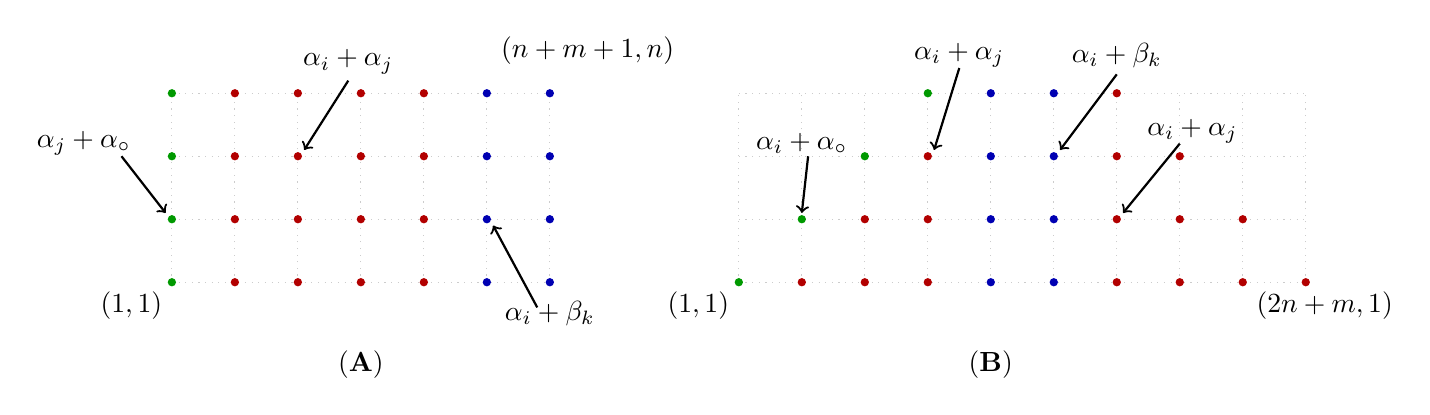
\begin{tikzpicture}[
    scale=0.8,
    dot/.style={circle,inner sep=0pt,minimum size=3pt},
    greenpt/.style={dot,fill=green!60!black},
    redpt/.style={dot,fill=red!70!black},
    bluept/.style={dot,fill=blue!70!black}
]

%==================== (A) full-space geometry ====================%
\begin{scope}
  % grid (dotted)
  \foreach \i in {0,...,6}{
    \draw[gray!40,dotted] (\i,0) -- (\i,3);
  }
  \foreach \j in {0,...,3}{
    \draw[gray!40,dotted] (0,\j) -- (6,\j);
  }

  % green column (left)
  \foreach \j in {0,...,3}{
    \node[greenpt] at (0,\j) {};
  }

  % red bulk columns
  \foreach \i in {1,...,4}{
    \foreach \j in {0,...,3}{
      \node[redpt] at (\i,\j) {};
    }
  }

  % blue columns (right)
  \foreach \i in {5,6}{
    \foreach \j in {0,...,3}{
      \node[bluept] at (\i,\j) {};
    }
  }

  % labels (1,1) and (n,n+m+1)
  \node[below left] at (0,0) {$(1,1)$};
  \node[above] at (6.6,3.3) {$(n+m+1,n)$};

  % parameter labels with arrows
  \node at (-1.4,2.2) {$\alpha_j+\alpha_{\circ}$};
  \draw[->,thick] (-0.8,2.0) -- (-0.1,1.1);

  \node at (2.8,3.5) {$\alpha_i+\alpha_j$};
  \draw[->,thick] (2.8,3.2) -- (2.1,2.1);

  \node at (6,-0.5) {$\alpha_i+\beta_k$};
  \draw[->,thick] (5.8,-0.4) -- (5.1,0.9);

  % subfigure label (A)
  \node at (3,-1.3) {(\textbf{A})};
\end{scope}

%==================== (B) trapezoidal / half-space geometry ======%
\begin{scope}[xshift=9cm]
  % dotted grid big enough for trapezoid
  \foreach \i in {0,...,9}{
    \draw[gray!40,dotted] (\i,0) -- (\i,3);
  }
  \foreach \j in {0,...,3}{
    \draw[gray!40,dotted] (0,\j) -- (9,\j);
  }

  % green boundary (diagonal-ish)
  \foreach \p in {(0,0),(1,1),(2,2),(3,3)}{
    \node[greenpt] at \p {};
  }

  % red region (left/right)
  % left small staircase
  \foreach \p in {(1,0),(2,0),(2,1),(3,0),(3,1),(3,2),(6,1),(6,2),(6,3),(6,0),(7,1),(7,2),(7,0),(8,1),(9,0),(8,0)}{
    \node[redpt] at \p {};
  }

% labels (1,1) and (n,n+m+1)
  \node[below left] at (0,0) {$(1,1)$};
  \node[below] at (9.3,0) {$(2n+m,1)$};

  % central blue strip
  \foreach \i in {4,5}{
    \foreach \j in {0,...,3}{
      \node[bluept] at (\i,\j) {};
    }
  }

  % parameter labels with arrows
  \node at (1,2.2) {$\alpha_i+\alpha_{\circ}$};
  \draw[->,thick] (1.1,2) -- (1,1.1);

  \node at (3.5,3.6) {$\alpha_i+\alpha_j$};
  \draw[->,thick] (3.5,3.4) --(3.1,2.1);

  \node at (6,3.6) {$\alpha_i+\beta_k$};
  \draw[->,thick] (6, 3.3) --(5.1,2.1);

  \node at (7.2,2.4) {$\alpha_i+\alpha_j$};
  \draw[->,thick] (7.0,2.2) --(6.1,1.1);

  % subfigure label (B)
  \node at (4,-1.3) {(\textbf{B})};
\end{scope}

\end{tikzpicture}
\caption{Parameter configuration for the Barraquand--Wang log-gamma polymers:
(A) full-space point-to-point geometry, (B) octant/trapezoidal geometry.}
\label{fig:BW-geometry}
\end{figure}


%%%%%%%%%%%%%%%%%%%%%%%%%%%%%%%%%%%%%%%%%%%%%%%%%%%%%%%%%%%%%%%%%%%%%
%  Full-space partition function
%%%%%%%%%%%%%%%%%%%%%%%%%%%%%%%%%%%%%%%%%%%%%%%%%%%%%%%%%%%%%%%%%%%%%
\begin{theorem}\label{thm:BW}
Fix $n,m\in\mathbb{N}$, and parameters
\[
\alpha^{\circ}>0,\qquad 
\alpha=(\alpha_1,\dots,\alpha_n)\in(\mathbb{R}_{>0})^n,\qquad
\beta=(\beta_1,\dots,\beta_m)\in(\mathbb{R}_{>0})^m,
\]
satisfying the compatibility conditions
\[
\alpha_i+\alpha^{\circ}>0,\qquad
\alpha_i+\alpha_j>0,\qquad
\alpha_i+\beta_k>0,
\]
for all $1\leq i,j \leq n$ and $1 \leq k \leq m$. Let all polymer weights be independent inverse-gamma 
random variables with the shape parameters described below.

\paragraph{Full-space point-to-point model.}
Consider the following rectangular domain
\[
\{(i,j): 1 \leq i \leq n+m+1, 1 \leq j \leq n\}.
\]
For $(i,j)$ in this rectangular domain, set
\[
W_{i,j}\sim
\begin{cases}
\mathrm{Gamma}^{-1}(\alpha_j+\alpha^{\circ}), & i=1,\\[3pt]
\mathrm{Gamma}^{-1}(\alpha_{i-1}+\alpha_{j}),   & 2\le i\le n+1,\\[3pt]
\mathrm{Gamma}^{-1}(\alpha_j+\beta_{i-n-1}), & n+2\le i\le n+m+1,
\end{cases}
\]
all independent and define the point-to-point partition function
\[
Z_1(n+m+1;n)
=\sum_{\pi\in\Pi[(1,1)\to(n+m+1,n)]}
\prod_{(i,j)\in\pi} W_{i,j}.
\]



\paragraph{Half-space point-to-line model.}
Consider the following trapezoidal domain
\[
\bigl\{(i,j)\in\mathbb{Z}^2: 
1\le j\le n,\ 
j\le i\le 2n+m-j+1 \bigr\}.
\]
For $(i,j)$ in this trapezoidal domain, set
\[
M_{i,j}\sim
\begin{cases}
\mathrm{Gamma}^{-1}(\alpha_i+\alpha^{\circ}), & 1\le i=j\le n,\\[3pt]
\mathrm{Gamma}^{-1}(\alpha_i+\alpha_j),      & 1\le j<i\le n,\\[3pt]
\mathrm{Gamma}^{-1}(\alpha_j+\beta_{i-n}),   & 1\le j\le n,\ n<i\le n+m,\\[3pt]
\mathrm{Gamma}^{-1}(\alpha_j+\alpha_{2n+m-i+1}), 
& 1\le j\le n,\ n+m<i\le 2n+m-j+1.
\end{cases}
\]
all independent and define the half-space point-to-line partition function
\[
Z_2(n+m+1;n)=\sum_{k=1}^n \sum_{\pi \in \Pi_{\HH}[(1,1) \to (2n-k+m+1,k)]} \prod_{(i,j) \in \pi} M_{i,j}
\]
With the above parameterization of inverse-gamma weights, the half-space
point-to-line partition function has the same law as the 
full-space point-to-point partition function:
\[
Z_1(n+m+1;n)\;\stackrel{d}{=}\;Z_2(n+m+1;n).
\]
\end{theorem}


By Theorem \ref{thm:BW}, we see that the following proposition implies Proposition \ref{prop:uniform_upper_tail}. 

\begin{proposition}\label{prop:inhomo_full_space}
    Fix $\alpha,\kappa > 0$ and $\theta \geq 0$. Let $Z_\theta(N,T)$ be the full-space log-gamma point-to-point partition function from
$(1,1)$ to $(N,T)$ with independent weights
$W_{i,j}\sim\mathrm{Gamma}^{-1}(A_i+B_j)$, where
$A_1=\theta$, $A_2=\cdots=A_N=\alpha$, and
$B_1=\cdots=B_T=\alpha$. There exists some positive constants $N_0, C, c$ such that for all $N \geq N_0$ and $T \geq 1$ satisfying $T/N \in (0, 1-\kappa N^{-1/3+\delta}]$ and all $x \geq 0$, we have
    \begin{equation}
        \Prob\left(\log Z_\theta(N,T) + Nf\left(T/N\right) \geq xN^{1/3}\right) \leq CNe^{-c \min \{N^{2\delta}, N^{1/3}\}} + CNe^{-cx^2}.
    \end{equation}  
\end{proposition}

This is because if we specialize the parameters in Theorem \ref{thm:BW}:
\[
\alpha^{\circ} = \theta; \quad \alpha_1 = \alpha_2 = \cdots = \beta_1 = \beta_2 = \cdots = \alpha
\]
Then
\begin{equation}
    \begin{aligned}
        &\Prob\left( \log \Zhalf(N,T)  \geq x\right) \leq \Prob\left( \log Z_2(N;T) \geq x \right) = \Prob\left( \log Z_\theta(N,T) \geq x\right).  
    \end{aligned}
\end{equation}

\subsection{Homogeneous full-space estimates}
Before proving Proposition \ref{prop:inhomo_full_space}, we need few results from the homogeneous full-space model. We want to first introduce the following homogeneous full-space upper-tail estimate, proved in \cite[Theorem~1.7]{barraquand2021fluctuations} via a steepest-descent analysis of the associated Fredholm determinant.
\begin{theorem}\label{thm:full-homogeneous}
    Fix any $\alpha > 0$ and $\xi \in (0,1)$. There exists some positive constants $N_0, C_1,C_2, c_1,c_2$ depending only on $\alpha,\xi$ such that for all $N \geq T \geq N_0$ satisfying $T/N \in [\xi, 1]$ and all $x \geq 0$, we have
    \begin{equation}
        \Prob\left(\log \Zfull(N,T) + Nf\left(T/N\right) \geq xN^{1/3}\right) \leq C_1e^{-c_1N} + C_2 e^{-c_2x^{3/2}}.
    \end{equation}  
\end{theorem}


We now turn to the complementary {thin-rectangle} regime $T/N\ll 1$, where a simpler estimate suffices.
\begin{proposition}\label{prop:thin-rect}
    For any $\varepsilon > 0$, there exists a $\xi \in (0,1)$ and positive constants $N_0, c$ such that for all $N \geq N_0$ satisfying $T/N \in (0, \xi]$ and all $x \geq 0$, we have
    \begin{equation}\label{eq:thin_rect}
        \Prob\left(\log \Zfull(N,T) + (N+T-1)\Psi_0(2\alpha-\varepsilon)\geq x \right) \leq e^{-cx}.
    \end{equation}  
\end{proposition}

\begin{proof}
Recall that for $\lambda \in (0,1)$, we have
\begin{equation}\label{eq:ineq}
\Zfull(N,T)^\lambda =\left( \sum_{\pi \in \Pi[(1,1) \rightarrow (N,T)]} \prod_{v \in \pi} w_v\right)^\lambda \leq \sum_{\pi \in \Pi[(1,1) \rightarrow (N,T)]} \prod_{v \in \pi} w_v^\lambda.
\end{equation}
Recall that if $w \sim \mathrm{Gamma}^{-1}(\beta)$ and $\beta-\lambda > 0$,
\[
\E[w^\lambda] = \frac{\Gamma(\beta - \lambda)}{\Gamma(\beta)}.
\] 
For $\lambda < \min\{1, 2\alpha\}$, we take expectation on both sides of \eqref{eq:ineq} and use independence along each path
\[
\E[\Zfull(N,T)^\lambda] \leq \binom{N+T-2}{N-1}\left( \frac{\Gamma(2\alpha -\lambda)}{\Gamma(2\alpha)}\right)^{N+T-1}.
\]
By Markov, we know that
\[
\begin{split}
    \Prob\left( \log \Zfull(N,T) \geq u \right)\leq \exp\left(-\lambda u + \log \binom{N+T-2}{N-1}+ (N+T-1)\log \left(\frac{\Gamma(2\alpha - \lambda)}{\Gamma(2\alpha)} \right) \right).
\end{split}
\]
Thus,
\[
\begin{split}
    &\Prob\left( \log \Zfull(N,T) - \frac{1}{\lambda} \log \binom{N+T-2}{N-1}-\frac{(N+T-1)}{\lambda} \log \left(\frac{\Gamma(2\alpha - \lambda)}{\Gamma(2\alpha)} \right) \geq x \right) \leq e^{-\lambda x}.
\end{split}
\]
Notice that for $\lambda$ small enough, we have
\[
\frac{1}{\lambda}\log\frac{\Gamma(2\alpha - \lambda)}{\Gamma(2\alpha)} \approx -\Psi_0(2\alpha).
\]
Recall that $-\Psi_0$ is a strictly decreasing function. Let $L = -\Psi_0(2\alpha-\varepsilon) + \Psi_0(2\alpha) > 0$. Let us choose $\lambda$ small such that 
\[
\left|\frac{1}{\lambda}\log\frac{\Gamma(2\alpha - \lambda)}{\Gamma(2\alpha)} + \Psi_0(2\alpha)\right| < \frac{L}{2}.
\]
Thus,
\[
\begin{aligned}
 -\frac{(N+T-1)}{\lambda}\log\frac{\Gamma(2\alpha - \lambda)}{\Gamma(2\alpha)} &\geq (N+T-1)\Psi_0(2\alpha) - (N+T-1)L/2\\
&= (N+T-1)\Psi_0(2\alpha-\varepsilon) + (N+T-1)L/2
\end{aligned}
\]
By Stirling's formula, we see that
\[
\log \binom{N+T-2}{N-1} =\left( \left(1+\frac{T}{N}\right)\log \left(1+\frac{T}{N}\right) -  \left(\frac{T}{N}\right)\log\left(\frac{T}{N}\right) \right) N + \mathcal{O}(\log N)
\]
Let us choose $\xi$ small enough such that 
\[
(1+\xi)\log(1+\xi)-\xi\log(\xi) < L\lambda/2.
\]
Thus, 
\[
- \frac{1}{\lambda} \log \binom{N+T-2}{N-1}-\frac{(N+T-1)}{\lambda} \log \left(\frac{\Gamma(2\alpha - \lambda)}{\Gamma(2\alpha)} \right) \geq (N+T-1)\Psi_0(2\alpha-\varepsilon).
\] 
We can then conclude
\[
\begin{split}
&\Prob\left( \log \Zfull(N,T) +(N+T-1)\Psi_0(2\alpha-\varepsilon) \geq x \right)\\
    &\leq \Prob\left( \log \Zfull(N,T) - \frac{1}{\lambda} \log \binom{N+T-2}{N-1} -\frac{(N+T-1)}{\lambda} \log \left(\frac{\Gamma(2\alpha - \lambda)}{\Gamma(2\alpha)} \right) \geq x \right)\\
    &\leq e^{-\lambda x}.
\end{split}
\]
\end{proof}

\subsection{Inequalities of shape function}
\begin{lemma}\label{lem:shape_linear_bound}
Fix $\alpha,\kappa>0$ and recall
\[
g(\zeta)=\frac{\Psi_1(2\alpha-\zeta)}{\Psi_1(\zeta)},\qquad 
f(x)=x\,\Psi_0(g^{-1}(x))+\Psi_0\bigl(2\alpha-g^{-1}(x)\bigr).
\]
Then there exist some $N_0,C_0 > 0$ depending on $\alpha,\kappa$ such that for any $N \geq N_0$, $T/N\in(0,1 - \kappa N^{-1/3+\delta}]$, and every $k\in\{1,\dots,T\}$,
\begin{equation}\label{eq:strict_shape_ineq}
-Nf\left( \frac{T}N\right)\;\geq \;-Nf\!\left(\frac{T-k}{N}\right)-k\,\Psi_0(\alpha) + C_0kN^{-1/3+\delta}.
\end{equation}
\end{lemma}
\begin{proof}
Write $\zeta(x)=g^{-1}(x)$. Differentiating
\[
f(x)=x\,\Psi_0(\zeta(x))+\Psi_0(2\alpha-\zeta(x))
\]
gives
\[
f'(x)=\Psi_0(\zeta(x))+\Bigl(x\Psi_1(\zeta(x))-\Psi_1(2\alpha-\zeta(x))\Bigr)\zeta'(x).
\]
Since $x=g(\zeta(x))=\Psi_1(2\alpha-\zeta(x))/\Psi_1(\zeta(x))$, the bracket vanishes and hence
\begin{equation}\label{eq:fprime}
f'(x)=\Psi_0(\zeta(x))=\Psi_0(g^{-1}(x)).
\end{equation}
Recall that $g^{-1}$ is strictly increasing on $(0,2\alpha)$ and $\Psi_0$ is strictly increasing on $(0,\infty)$. Thus,
\[
f'(x)=\Psi_0(g^{-1}(x))<\Psi_0(g^{-1}(1)) = \Psi_0(\alpha),\qquad x\in(0,1).
\]
By the mean value theorem, there exists
$s\in(\frac{T-k}{N},\frac{T}{N})\subset(0,1-\kappa N^{-1/3+\delta}]$ such that
\[
f\left(\frac{T}{N}\right)-f\left(\frac{T-k}{N}\right)=f'(s)\frac{k}{N}
\]
Notice that 
\[
\alpha - g^{-1}(s) \geq \alpha- g^{-1}\left(1-\kappa N^{-1/3+\delta}\right) \geq C_1N^{-1/3+\delta}
\]
for some $C_1 > 0$ by Proposition \ref{prop:slope}. Because $\Psi_0$ is strictly concave on $(0, \infty)$, we have
\[
\Psi_0(\alpha) - \Psi_0(g^{-1}(s)) \geq C_1\Psi_1(\alpha)N^{-1/3+\delta}.
\]
Lastly, we have
\[
\frac{k}{N}\Psi_0(\alpha) - f\left(\frac{T}{N}\right)+f\left(\frac{T-k}{N}\right) \geq \frac{k}{N}C_1\Psi_1(\alpha)N^{-1/3+\delta}.
\]
Multiplying $N$ on both sides yields the desired inequality.
\end{proof}

\begin{lemma}\label{lem:shape_rect_bound}
Fix $\alpha, \kappa > 0$. There exists some $N_0, C_0 > 0$ depending on $\alpha, \kappa$ such that for any $N \geq N_0$, $T/N\in(0,1 - \kappa N^{-1/3+\delta}]$, and every $k\in\{1,\dots,T\}$, we have
\begin{equation}\label{eq:strict_shape_ineq}
-Nf\left( \frac{T}N\right)\;\geq \;-(N+T-k)\Psi_0(3\alpha/2)-k\,\Psi_0(\alpha) + C_0N.
\end{equation}
\end{lemma}

\begin{proof}

Recall that $-Nf(T/N) = (N+T)F(g^{-1}(T/N))$ where 
\[
F\left(\zeta \right) = -  \frac{\Psi_1(2\alpha - \zeta)}{\Psi_1(\zeta) + \Psi_1(2\alpha - \zeta)}\Psi_0(\zeta) - \frac{\Psi_1(\zeta)}{\Psi_1(\zeta) + \Psi_1(2\alpha-\zeta)}\Psi_0(2\alpha - \zeta).
\]
By Proposition \ref{prop:slope}, we know that
\[
\alpha- g^{-1}\left(\frac{T}{N}\right) \geq C_1\kappa N^{-1/3 + \delta}
\]
for some $C_1 > 0$. Thus, by Proposition \ref{prop:shape}, we have
\[
\left|F(\alpha) - F\left( g^{-1}\left(\frac{T}{N} \right)\right) \right| \geq C_2 N^{-2/3 + 2\delta}
\]
for some $C_2 > 0$. Since $F(\alpha) = -\Psi_0(\alpha)$,
\[
\begin{aligned}
&(N+T)F\left( g^{-1}\left(\frac{T}{N} \right)\right) \geq (N+T)F(\alpha) - C_2 (N+T) N^{-2/3 + 2\delta}\\
&= -k\Psi_0(\alpha) - (N+T-k)\Psi_0(3\alpha/2) +(N+T-k)(\Psi_0(3\alpha/2)-\Psi_0(\alpha))- C_2 (N+T) N^{-2/3 + 2\delta}.
\end{aligned}
\]
Because $\Psi_0$ is strictly increasing on $(0, \infty)$, $\Psi_0(3\alpha/2) - \Psi_0(\alpha) >0$ and we can choose $N_0$ large enough so that $C_2 (N+T) N^{-2/3 + 2\delta}$ gets absorbed into $(N+T-k)(\Psi_0(3\alpha/2)-\Psi_0(\alpha))$.

\end{proof}


\subsection{Proof of Proposition \ref{prop:inhomo_full_space}}
\begin{proof}[Proof of Proposition \ref{prop:inhomo_full_space}]
By \cite[Lemma 13.1]{stat}, we know that $Z_0(N,T)$ stochastically dominates $Z_\theta(N,T)$ for all $\theta \geq 0$. Thus, it suffices to only prove the upper tail for $\theta=0$. Write 
\[
Z_0(N,T) = \sum_{k=1}^{T} \left( \prod_{j=1}^k W_{1,j} \right)\Zfull(2,k;N,T).
\]
Thus,
\[
\log Z_0(N,T) \leq \log T + \max_{1 \leq k\leq T}\left\{  \sum_{j=1}^k \log W_{1,j}+ \log\Zfull(2,k;N,T)\right\}.
\]
It suffices to prove for all $1 \leq k \leq T$,
\[
\Prob\left(\sum_{j=1}^k \log W_{1,j}+ \log\Zfull(2,k;N,T) + Nf(T/N) \geq xN^{1/3}\right) \leq Ce^{-c \min \{N^{2\delta}, N^{1/3}\}} + Ce^{-cx^2}
\]
because
\[
\begin{aligned}
    &\Prob\left(\log Z_0(N,T) + Nf\left(T/N\right) \geq xN^{1/3}\right) \\
    &\leq \Prob\left( \max_{1 \leq k\leq T}\left\{  \sum_{j=1}^k \log W_{1,j}+ \log\Zfull(2,k;N,T)\right\} + Nf\left(T/N\right) \geq xN^{1/3} - \log T\right)\\
    &\leq T \max_{1 \leq k\leq T}\Prob\left(\sum_{j=1}^k \log W_{1,j}+ \log\Zfull(2,k;N,T) + Nf\left(T/N\right) \geq xN^{1/3} - \log T\right)\\
    &\leq CNe^{-c \min \{N^{2\delta}, N^{1/3}\}} + CNe^{-cx^2}.
\end{aligned}
\]
Choose $\xi$ in Proposition \ref{prop:thin-rect} by setting $\varepsilon = \alpha/2$. We consider the first case where $k \geq T-\xi N$. We apply Lemma \ref{lem:shape_rect_bound}:
\[
\begin{aligned}
&\Prob\left(\sum_{j=1}^k \log W_{1,j}+ \log\Zfull(2,k;N,T) + Nf(T/N) \geq xN^{1/3}\right)\\
&\leq \Prob\left(\sum_{j=1}^k \log W_{1,j}+ k\Psi_0(\alpha) \geq C_0N\right) + \Prob \left(\log\Zfull(2,k;N,T) + (N+T-k)\Psi_0(3\alpha/2) \geq xN^{1/3}\right).
\end{aligned}
\]
Apply Bernstein inequality for subexponential random variables \cite[Theorem 2.9.1]{Vershynin_2018} and Proposition \ref{prop:thin-rect}, we see that the above is bounded by $Ce^{-cN^{1/3}}$.

Consider the second case where $1 \leq k \leq T - \xi N$. We apply Lemma \ref{lem:shape_linear_bound}:
\[
\begin{aligned}
&\Prob\left(\sum_{j=1}^k \log W_{1,j}+ \log\Zfull(2,k;N,T) + Nf(T/N) \geq xN^{1/3}\right)\\
&\leq \Prob\left(\sum_{j=1}^k \log W_{1,j}+ k\Psi_0(\alpha) \geq C_0kN^{-1/3+\delta} + \frac{xN^{1/3}}{2}\right) + \Prob \left(\log\Zfull(2,k;N,T) + Nf((T-k)/N) \geq \frac{xN^{1/3}}{2}\right).
\end{aligned}
\]
We apply Theorem \ref{thm:full-homogeneous} with the $\xi$ chosen above to the second term and bound it by $Ce^{-cx^{3/2}}$. For the first term, we want to apply Bernstein inequality. If $k \leq N^{2/3}$, then the first term is bounded by $Ce^{-cx^2}$. If $k \geq N^{2/3}$, then $kN^{-2/3+2\delta} \geq N^{2\delta}$ and the first term is bounded by $Ce^{-c\min\{N^{2\delta},N^{1/3+\delta}\}}$. Note that all the constants $C,c>0$ only depend on $\alpha$ and $\kappa$.

\end{proof}



\section{Acknowledgments}
The author sincerely thanks their advisor, Ivan Corwin, for constant support and guidance. The author is especially grateful to Sayan Das for suggesting this problem and for valuable discussion on the uniform exponential upper-tail bounds for the half-space free energy with general slope. The author also thanks Jiyue Zeng and Alan Zhao for valuable conversations. This research was partially supported by Ivan Corwin’s National Science Foundation grant DMS:2246576 and Simons Investigator in Mathematics award MPS-SIM-00929852.
\bibliographystyle{amsalpha}
\bibliography{bib.bib}
\end{document}
